\section{问题三模型的建立与求解}

\subsection{建模思路}

问题三与问题二相比，微网物理结构没有改变，变化的是日内信息集。问题二每天只在 0:00 制定一次全天计划；问题三在 0:00、6:00、12:00、18:00 均可获得新的未来 24 h 光伏预报，因此可以对尚未执行时段的正常购电计划进行滚动修正。

问题三继续沿用问题二中的基础物理变量 \(G^L,\ G^{ch},\ PV^{ch},\ C,\ D,\ E,\ V,\ W,\ H,\ u\)， 并保留 7 日滚动 SAA 框架。新增变量来自“原计划—阶段调整—最终生效计划”的业务关系：

\begin{itemize}
\item \(P_{d,t}\)：0:00 原始计划；
\item \(A^s_{d,t}\)：阶段 \(s\in\{6,12,18\}\) 重新优化后的计划；
\item \(B_{d,t}\)：将各阶段真实生效区间拼接后的最终全天计划；
\item \(\Delta^+,\Delta^-\)：最终计划相对 0:00 原计划的调增量和调减量。
\end{itemize}

因此问题三可以概括为

\[
\boxed{
Q3
=
Q2\text{ 正式模型}
+
0/6/12/18\text{ 光伏预报更新}
+
\text{购电计划再调整}
}.
\]

\subsection{时间与信息结构}

每天划分为 \(T=144,, \Delta t=\frac16\ \mathrm{h}\)。 阶段集合为

\[
\mathcal S=\{0,6,12,18\}.
\]

0:00 可决定全天计划，6:00 以后只能重新决定 6:00—24:00，12:00 以后只能重新决定 12:00—24:00，18:00 以后只能重新决定 18:00—24:00。已经执行的历史时段永久锁定。

0:00 时允许使用历史真实负荷、历史真实光伏、历史附件 3 预报、当天 0:00 最新光伏预报和当前真实储电量；不得使用当天未来真实负荷、真实光伏和尚未发布的后续预报。

6:00、12:00、18:00 时，可以新增使用已经发生时段的真实负荷、真实光伏、当前真实储电量以及当前最新附件 3 预报，但仍不得读取当前时刻之后的真实值。

2025 年 1 月继续作为预热期，正式报送窗口为 2025 年 2 月 1 日至 12 月 31 日。

\subsection{负荷与光伏预测}

问题三没有提供新的负荷预报，因此每天 0:00 仍使用问题二的负荷预测模型产生未来 7 日中心预测 \(\hat L_{\tau,t}^{(d)},, \tau=d,\ldots,d+6\)。 同一天 6:00、12:00、18:00 不重新训练负荷预测。

对于光伏，在阶段 \(s\in\{0,6,12,18\}\) 将附件 3 当前阶段最新发布的未来 24 h 预测作为近端中心预测，记为 \(\widehat{PV}^{(d,s)}\)。 发布时刻 \(\tau\) 的第 \(k\) 小时预报对应 \([\tau+(k-1)\mathrm{h},\tau+k\mathrm{h})\)。 附件 3 为整点预测，而调度粒度为 10 min，因此采用线性插值：

\begin{equation}
F_{h,m}
=
F_h+\frac{m}{6}(F_{h+1}-F_h),
\qquad
m=0,\ldots,5.
\end{equation}

同一未来时段若存在多版预测，只使用当前时刻最新已发布版本，即新预报覆盖旧预报。

官方预报只覆盖未来 24 h，超过 24 h 后为维持 7 日滚动视野，继续采用问题二自建光伏预测。

\subsection{光伏预报误差与 SAA 情景}

附件 3 给出的仍是预报而不是真值，因此不能把最新预报直接作为确定性未来光伏。

负荷残差继续采用

\[
e^L_{r,t}
=
L^{act}_{r,t}
-
\hat L_{r,t}.
\]

针对四个发布阶段分别建立光伏预报误差库：

\[
\mathcal E_{PV}^{0},
\quad
\mathcal E_{PV}^{6},
\quad
\mathcal E_{PV}^{12},
\quad
\mathcal E_{PV}^{18}.
\]

阶段 \(s\) 的历史光伏预报残差为

\begin{equation}
e^{PV,s}_{r,\ell}
=
PV^{act}_{r,\ell}
-
\widehat{PV}^{s}_{r,\ell}.
\end{equation}

残差按预测提前量对齐，并使用最近 28 个有效历史日。负荷与光伏残差尽量从同一历史日期联合抽取。

正式取 \(K=4\)， 稳定性分析取 \(K=8\)， 随机种子为 2026。

第 \(\omega\) 个负荷情景为

\begin{equation}
L^{(\omega)}_{\tau,t}
=
\max
\left\{
0,
\hat L^{(d)}_{\tau,t}
+
e^L_{r_\omega,t}
\right\},
\end{equation}

近端 24 h 光伏情景为

\begin{equation}
PV^{(\omega)}_{\tau,t}
=
\max
\left\{
0,
\widehat{PV}^{(d,s)}_{\tau,t}
+
e^{PV,s}_{r_\omega,\ell}
\right\}.
\end{equation}

24 h 以后则采用问题二光伏预测及其历史误差生成情景。

\subsection{7 日滚动视野}

阶段 \(s\) 的优化窗口为

\begin{equation}
\mathcal H_{d,s}
=
\text{当天尚未执行时段}
+
d+1,\ldots,d+6.
\end{equation}

即每次重新优化仍保留 7 日视野，但只执行当前阶段到下一更新阶段之间的部分。未来日期的计划仅用于估计延续成本，不代表真正提前提交未来计划。

\subsection{计划变量与调整结算}

0:00 原始计划为 \(P_{d,t}\ge0\)。 6:00、12:00、18:00 调整计划分别为

\begin{equation}
A^6_{d,t},
\qquad
A^{12}_{d,t},
\qquad
A^{18}_{d,t}.
\end{equation}

最终生效购电计划为

\begin{equation}
B_{d,t}
=
\begin{cases}
P_{d,t},&0\le t<6,\\
A^6_{d,t},&6\le t<12,\\
A^{12}_{d,t},&12\le t<18,\\
A^{18}_{d,t},&18\le t<24.
\end{cases}
\end{equation}

当前阶段计划变量在所有 SAA 情景中保持一致，以满足非预见性。

所有调整统一相对于当天 0:00 原始计划 \(P\) 结算，定义 \(B-P=\Delta^+-\Delta^-,, \Delta^+,\Delta^-\ge0\)。 正常购电及调整费用为

\begin{equation}
C^{normal}_{d,t}
=
\left[
\pi_tP_{d,t}
+
1.5\pi_t\Delta^+_{d,t}
-
0.5\pi_t\Delta^-_{d,t}
\right]\Delta t.
\end{equation}

多次临时调整不重复收费，只按最终生效计划 \(B\) 与 0:00 原始计划 \(P\) 之间的差额结算一次。

问题三电价始终为正，因此最优解中 \(\Delta^+\) 与 \(\Delta^-\) 不会同时为正，无需额外二元变量。

\subsection{物理执行变量与约束}

物理执行变量沿用问题二，物理约束的形式也与问题一、二逐条一致：负荷平衡、充电来源、
光伏剩余平衡仍为 \(G^L+D+H=\overline L\)、\(PV^{ch}+G^{ch}=C\)、\(PV^{ch}+V=\overline{PV}\)，
储能递推、储电量上下限、充放功率限制与充放电互斥亦不变。问题三新增的只是
\textbf{阶段内的计划锁定关系}：当前阶段尚未执行的购电量由该阶段的计划给出，并与实际执行量守恒，

\begin{equation}
G^L+G^{ch}+W=X^s,
\qquad
X^s=
\begin{cases}
P,&s=0,\\
A^s,&s=6,12,18,
\end{cases}
\end{equation}

其中 \(P\) 为 0:00 原始计划，\(A^s\) 为阶段 \(s\) 调整后的计划。每次进入新阶段重新求解时，
以真实执行后的储电量作为初值：

\begin{equation}
E^{(\omega)}_{d,s}=E^{act}_{d,s}.
\end{equation}

\subsection{目标函数}

0:00 阶段目标函数为

\begin{equation}
\min Z_{d,0}
=
\sum_t
\pi_tP_{d,t}\Delta t
+
\frac1K
\sum_{\omega}
\left[
\sum_t
5\pi_tH^{(\omega)}_{d,t}\Delta t
+
C^{future,(\omega)}
\right].
\end{equation}

6:00、12:00、18:00 阶段，设

\[
A^s-P
=
\Delta^{+,s}
-
\Delta^{-,s},
\]

则当前阶段调整结算费用为

\begin{equation}
C^{settle,s}_d
=
\sum_{t\ge s}
\left[
\pi_tP_{d,t}
+
1.5\pi_t\Delta^{+,s}_{d,t}
-
0.5\pi_t\Delta^{-,s}_{d,t}
\right]\Delta t.
\end{equation}

阶段 \(s\) 的优化目标为

\begin{equation}
\min Z_{d,s}
=
C^{settle,s}_d
+
\frac1K
\sum_{\omega}
\left[
C^{em,s,(\omega)}
+
C^{future,s,(\omega)}
\right].
\end{equation}

因此每次新预报到达后，模型都在“保持原计划”“支付调整成本”和“承担未来紧急购电风险”之间重新权衡。

\subsection{实际执行与滚动求解}

实际执行优先级为：

\begin{enumerate}
\item 实际光伏优先供实际负荷；
\item 当前生效正常购电补负荷；
\item 仍不足时储能放电；
\item 仍不足时紧急购电；
\item 负荷满足后光伏余电优先给储能充电；
\item 再用剩余正常购电给储能充电；
\item 剩余光伏记为 \(V\)；
\item 剩余已购正常电记为 \(W\)；
\item 同一时段不得同时充放电。
\end{enumerate}

模型经过 SAA 情景展开后仍属于 MILP，底层采用分支定界/分支切割方法，通过 MATLAB \texttt{intlinprog} 求解，并继续使用 LP 松弛热启动。

日内按四个时点推进：6:00、12:00 与 18:00 各重解一次，每次只对尚未执行的时段重新优化，求解完成后执行到下一个时点，如此推进至 24:00。

即每个阶段都重复“求解、执行、更新真实状态、再求解”的过程。

四阶段拼接得到最终生效计划 \(B\)，并可将 \(B\) 对全天真实数据完整重放一次，用于检查阶段滚动执行与最终拼接结果的一致性。

\subsection{预报时点组合与结果分析框架}

为判断是否需要引入全部三个额外预报时点，设置

\[
S_0=\{0\},
\quad
S_1=\{0,6\},
\quad
S_2=\{0,6,12\},
\quad
S_3=\{0,6,12,18\}.
\]

四种策略分别进行完整年度模拟。

\begin{table}[H]
\centering
\zihao{5}
\begin{tabular}{lrrrr}
\toprule
指标 & \(S_0\) & \(S_1\) & \(S_2\) & \(S_3\) \\
\midrule
总费用/元 & 15644696.18 & 15579634.76 & 15011622.48 & 14485230.30 \\
正常+调整费用/元 & 13020217.18 & 13323342.33 & 13231611.82 & 13451415.12 \\
紧急购电费用/元 & 2624479.00 & 2256292.43 & 1780010.65 & 1033815.18 \\
紧急购电量/kWh & 446736.83 & 367873.50 & 297408.27 & 185523.91 \\
调增购电量/kWh & 0.00 & 3154797.70 & 2742273.08 & 3452636.88 \\
调减购电量/kWh & 0.00 & 4390651.45 & 5260126.69 & 5431644.57 \\
弃光量/kWh & 1316638.95 & 1266813.04 & 1189640.51 & 1188715.64 \\
已购未用电/kWh & 1097272.92 & 835050.59 & 606925.45 & 601472.99 \\
\bottomrule
\end{tabular}
\caption{问题三四阶段策略典型日指标（费用单位：元，电量单位：kWh）}
\label{tab:8}
\end{table}

新增预报时点的边际收益定义为

\[
\Delta C_6=C(S_0)-C(S_1),
\]

\[
\Delta C_{12}=C(S_1)-C(S_2),
\]

\begin{equation}
\Delta C_{18}=C(S_2)-C(S_3).
\end{equation}

其中

\[
\Delta C_6=\text{65061.43 元},
\qquad
\Delta C_{12}=\text{568012.28 元},
\qquad
\Delta C_{18}=\text{526392.18 元}.
\]

结果分析时应重点判断：新增预报是主要降低了紧急购电、降低了已购未用电，还是仅增加调整频率而没有产生足够经济收益。

\begin{table}[H]
\centering
\zihao{5}
% 7 列，即使 tabcolsep 收到 4pt 仍超版心，整体缩放到版心宽
\resizebox{\textwidth}{!}{%
\begin{tabular}{lrrrrrr}
\toprule
日期 & 0:00计划购电/kWh & 最终调整购电/kWh & 紧急购电/kWh & 全天费用/元 & 日初储电量/kWh & 日末储电量/kWh \\
\midrule
2025-03-20 & 60456.54 & 59272.33 & 1042.42 & 41345.86 & 8924.47 & 3000.36 \\
2025-06-21 & 43252.47 & 42434.09 & 0.00 & 24946.99 & 5762.09 & 10800.00 \\
2025-09-23 & 65186.81 & 66030.22 & 1887.41 & 47560.08 & 4746.35 & 6520.75 \\
2025-12-21 & 96080.19 & 96520.33 & 0.00 & 63416.18 & 8821.22 & 8865.36 \\
\bottomrule
\end{tabular}}
\caption{问题三指定日期分阶段电量与费用（电量单位：kWh，费用单位：元）}
\label{tab:9}
\end{table}

%FIG:BEGIN q3-year
问题三逐日的购电与调整结构见图~\ref{fig:q3-year}。

\begin{figure}[htbp]
\centering
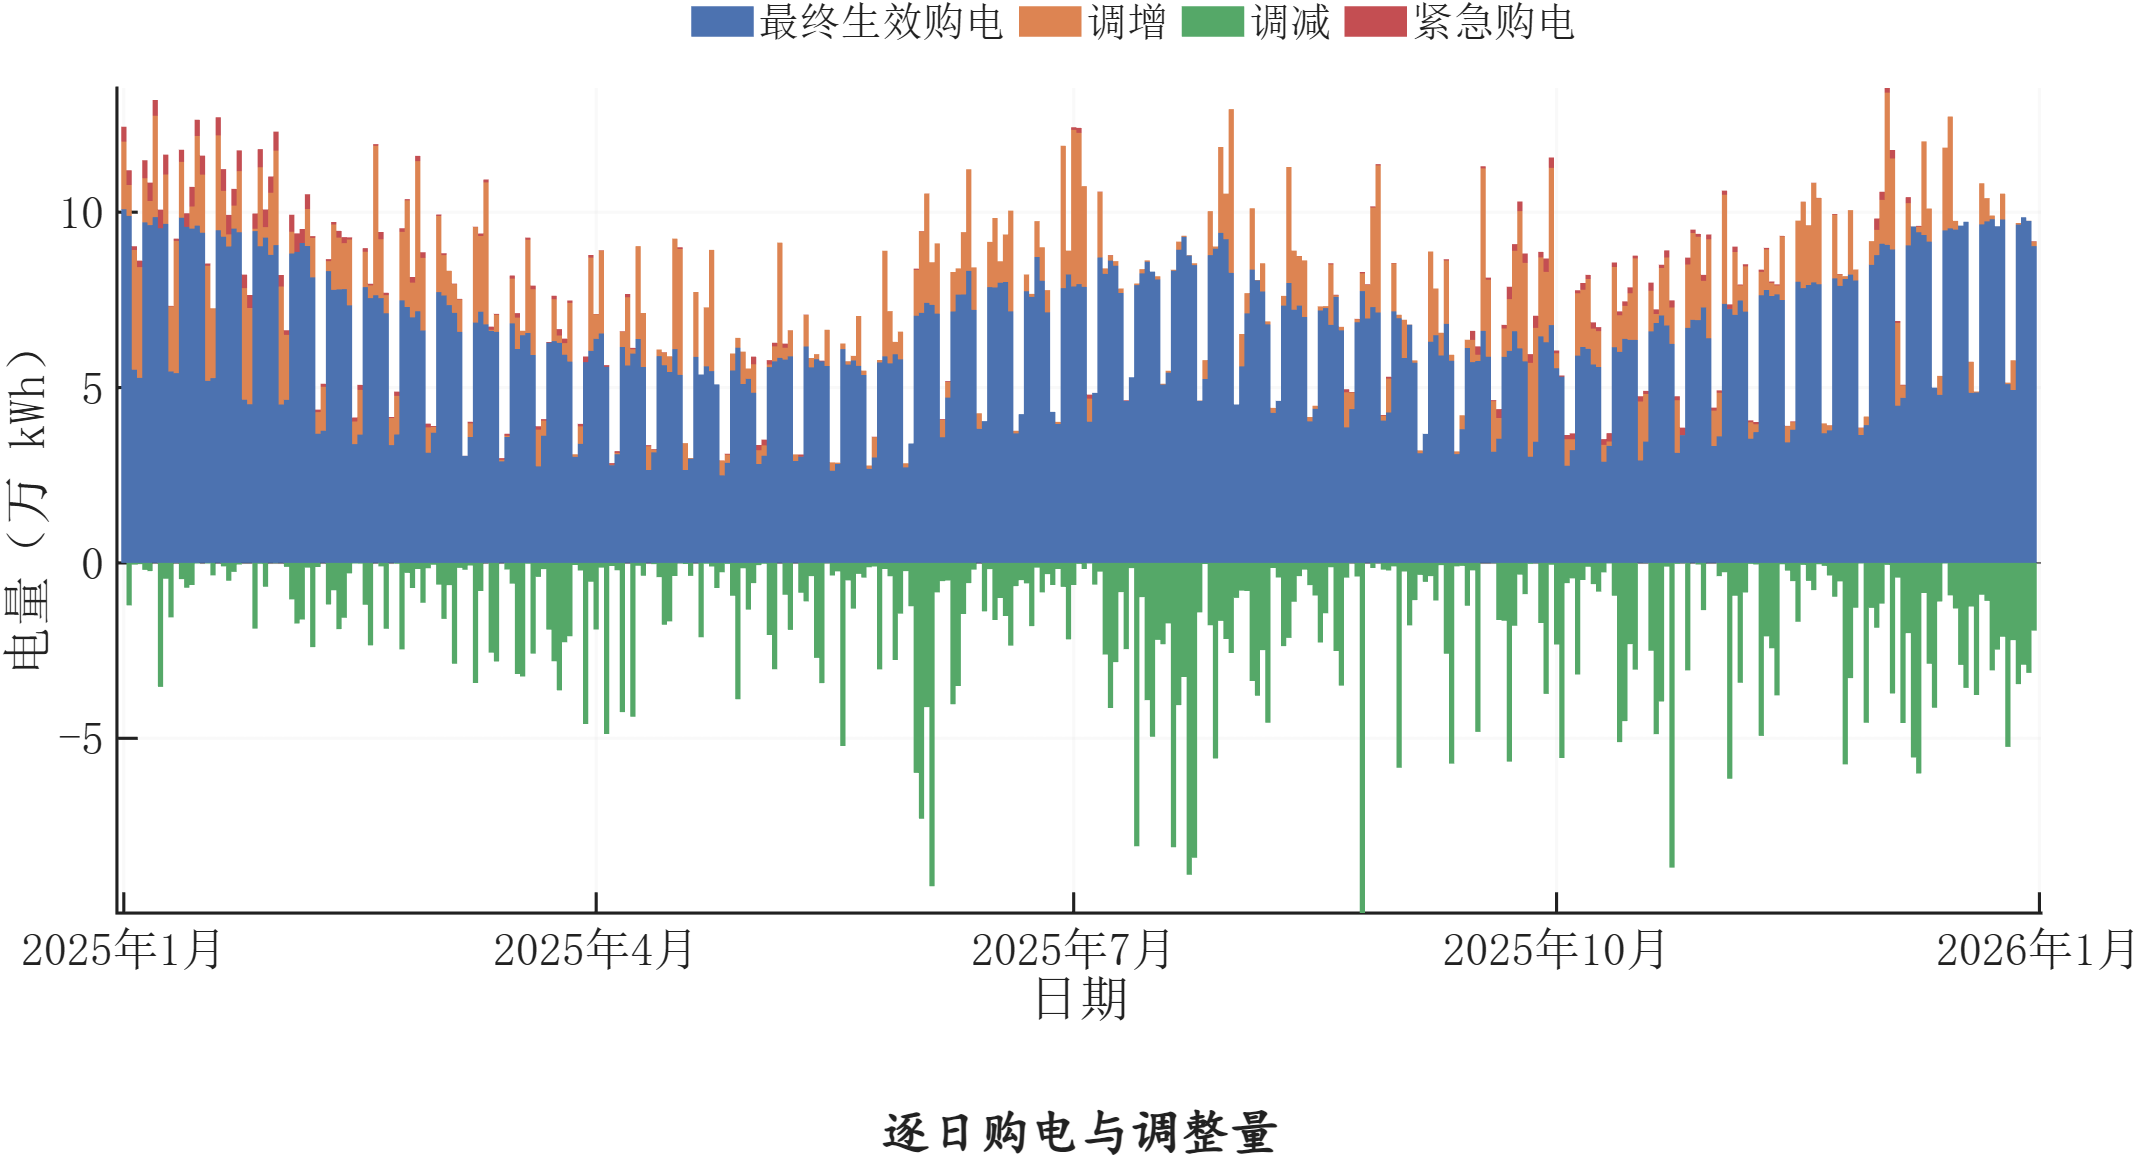
\includegraphics[width=0.78\textwidth,height=0.26\textheight,keepaspectratio]{figures/q3_year.png}
\caption{问题三逐日购电与调整结构（电量单位：kWh）}
\label{fig:q3-year}
\end{figure}

引入日内预报更新后，最终生效购电量仍逐日平稳，而调增与调减在大量日期发生：全年 339 天有调增、340 天有调减、225 天触发紧急购电，说明计划再调整已是常态机制。
%FIG:END q3-year
%MANDATED:BEGIN
按题目表 1、表 2 与表 3 要求的格式，四个指定日期的结果整理见后续横版页。

{\zihao{6}\setlength{\tabcolsep}{2pt}
\begin{center}
\begin{tabular}{|c|r|c|r|c|r|}
\hline
时间段 & 购电量/kWh & 时间段 & 购电量/kWh & 时间段 & 购电量/kWh \\
\hline
10:00-10:10 & \textbf{0.00} & 12:00-12:10 & \textbf{413.45} & 14:00-14:10 & \textbf{0.00} \\
\hline
16:00-16:10 & \textbf{543.44} & 18:00-18:10 & \textbf{710.86} & 20:00-20:10 & \textbf{0.00} \\
\hline
全天购电量 & \textbf{59272.33} & & & 全天购电费 & \textbf{41345.86} \\
\hline
\end{tabular}
\par{\zihao{6}表 1（2025.3.20）　问题三}

\vspace{0.15\baselineskip}
\begin{tabular}{|c|r|r|c|r|r|}
\hline
时间段 & 充电量/kWh & 放电量/kWh & 时间段 & 充电量/kWh & 放电量/kWh \\
\hline
0:00-4:00 & \textbf{1276.70} & \textbf{856.33} & 4:00-8:00 & \textbf{783.60} & \textbf{5541.40} \\
\hline
8:00-12:00 & \textbf{1481.27} & \textbf{2223.13} & 12:00-16:00 & \textbf{8982.23} & \textbf{254.72} \\
\hline
16:00-20:00 & \textbf{598.11} & \textbf{4992.86} & 20:00-24:00 & \textbf{2190.51} & \textbf{3866.32} \\
\hline
0:00 储电量 & \textbf{8924.47} & & 24:00 储电量 & \textbf{3000.36} & \\
\hline
\end{tabular}
\par{\zihao{6}表 2（2025.3.20）　问题三}

\vspace{0.15\baselineskip}
\begin{tabular}{|c|r|c|r|c|r|}
\hline
时间段 & 购电量/kWh & 时间段 & 购电量/kWh & 时间段 & 购电量/kWh \\
\hline
10:00-10:10 & \textbf{0.00} & 12:00-12:10 & \textbf{0.00} & 14:00-14:10 & \textbf{0.00} \\
\hline
16:00-16:10 & \textbf{68.84} & 18:00-18:10 & \textbf{487.84} & 20:00-20:10 & \textbf{0.00} \\
\hline
全天购电量 & \textbf{42434.09} & & & 全天购电费 & \textbf{24946.99} \\
\hline
\end{tabular}
\par{\zihao{6}表 1（2025.6.21）　问题三}

\vspace{0.15\baselineskip}
\begin{tabular}{|c|r|r|c|r|r|}
\hline
时间段 & 充电量/kWh & 放电量/kWh & 时间段 & 充电量/kWh & 放电量/kWh \\
\hline
0:00-4:00 & \textbf{1507.39} & \textbf{3.20} & 4:00-8:00 & \textbf{408.27} & \textbf{3472.44} \\
\hline
8:00-12:00 & \textbf{7972.94} & \textbf{0.00} & 12:00-16:00 & \textbf{0.00} & \textbf{0.00} \\
\hline
16:00-20:00 & \textbf{0.00} & \textbf{4097.93} & 20:00-24:00 & \textbf{8784.48} & \textbf{3017.50} \\
\hline
0:00 储电量 & \textbf{5762.09} & & 24:00 储电量 & \textbf{10800.00} & \\
\hline
\end{tabular}
\par{\zihao{6}表 2（2025.6.21）　问题三}

\vspace{0.15\baselineskip}
\begin{tabular}{|c|r|c|r|c|r|}
\hline
时间段 & 购电量/kWh & 时间段 & 购电量/kWh & 时间段 & 购电量/kWh \\
\hline
10:00-10:10 & \textbf{0.00} & 12:00-12:10 & \textbf{304.84} & 14:00-14:10 & \textbf{0.00} \\
\hline
16:00-16:10 & \textbf{475.56} & 18:00-18:10 & \textbf{628.02} & 20:00-20:10 & \textbf{103.69} \\
\hline
全天购电量 & \textbf{66030.22} & & & 全天购电费 & \textbf{47560.08} \\
\hline
\end{tabular}
\par{\zihao{6}表 1（2025.9.23）　问题三}

\vspace{0.15\baselineskip}
\begin{tabular}{|c|r|r|c|r|r|}
\hline
时间段 & 充电量/kWh & 放电量/kWh & 时间段 & 充电量/kWh & 放电量/kWh \\
\hline
0:00-4:00 & \textbf{5475.85} & \textbf{1065.44} & 4:00-8:00 & \textbf{1079.75} & \textbf{4742.01} \\
\hline
8:00-12:00 & \textbf{2130.33} & \textbf{2387.94} & 12:00-16:00 & \textbf{6835.16} & \textbf{471.71} \\
\hline
16:00-20:00 & \textbf{0.00} & \textbf{4953.17} & 20:00-24:00 & \textbf{6112.75} & \textbf{2306.17} \\
\hline
0:00 储电量 & \textbf{4746.35} & & 24:00 储电量 & \textbf{6520.75} & \\
\hline
\end{tabular}
\par{\zihao{6}表 2（2025.9.23）　问题三}

\vspace{0.15\baselineskip}
\begin{tabular}{|c|r|c|r|c|r|}
\hline
时间段 & 购电量/kWh & 时间段 & 购电量/kWh & 时间段 & 购电量/kWh \\
\hline
10:00-10:10 & \textbf{0.00} & 12:00-12:10 & \textbf{1031.99} & 14:00-14:10 & \textbf{0.00} \\
\hline
16:00-16:10 & \textbf{818.13} & 18:00-18:10 & \textbf{695.62} & 20:00-20:10 & \textbf{0.00} \\
\hline
全天购电量 & \textbf{96520.33} & & & 全天购电费 & \textbf{63416.18} \\
\hline
\end{tabular}
\par{\zihao{6}表 1（2025.12.21）　问题三}

\vspace{0.15\baselineskip}
\begin{tabular}{|c|r|r|c|r|r|}
\hline
时间段 & 充电量/kWh & 放电量/kWh & 时间段 & 充电量/kWh & 放电量/kWh \\
\hline
0:00-4:00 & \textbf{1762.08} & \textbf{54.41} & 4:00-8:00 & \textbf{1526.92} & \textbf{828.79} \\
\hline
8:00-12:00 & \textbf{3865.47} & \textbf{8085.13} & 12:00-16:00 & \textbf{8581.77} & \textbf{1997.13} \\
\hline
16:00-20:00 & \textbf{17.85} & \textbf{4961.30} & 20:00-24:00 & \textbf{8456.34} & \textbf{3643.97} \\
\hline
0:00 储电量 & \textbf{8821.22} & & 24:00 储电量 & \textbf{8865.36} & \\
\hline
\end{tabular}
\par{\zihao{6}表 2（2025.12.21）　问题三}

\vspace{0.15\baselineskip}
\begin{tabular}{|c|r|c|r|c|r|c|r|}
\hline
\multicolumn{2}{c|}{2025.3.20} & \multicolumn{2}{c|}{2025.6.21} & \multicolumn{2}{c|}{2025.9.23} & \multicolumn{2}{c|}{2025.12.21} \\
\hline
时间段 & 购电量/kWh & 时间段 & 购电量/kWh & 时间段 & 购电量/kWh & 时间段 & 购电量/kWh \\
\hline
8:50-10:10 & \textbf{1042.42} & 无 & \textbf{0.00} & 20:30-22:00 & \textbf{1887.41} & 无 & \textbf{0.00} \\
\hline
\end{tabular}
\par{\zihao{6}表 3　微网在指定日期的紧急购电量（问题三）}

\end{center}
}


%MANDATED:END

%FIG:BEGIN q3-stage
四个指定日期的四阶段计划轨迹见图~\ref{fig:q3-stage}。

\begin{figure}[htbp]
\centering
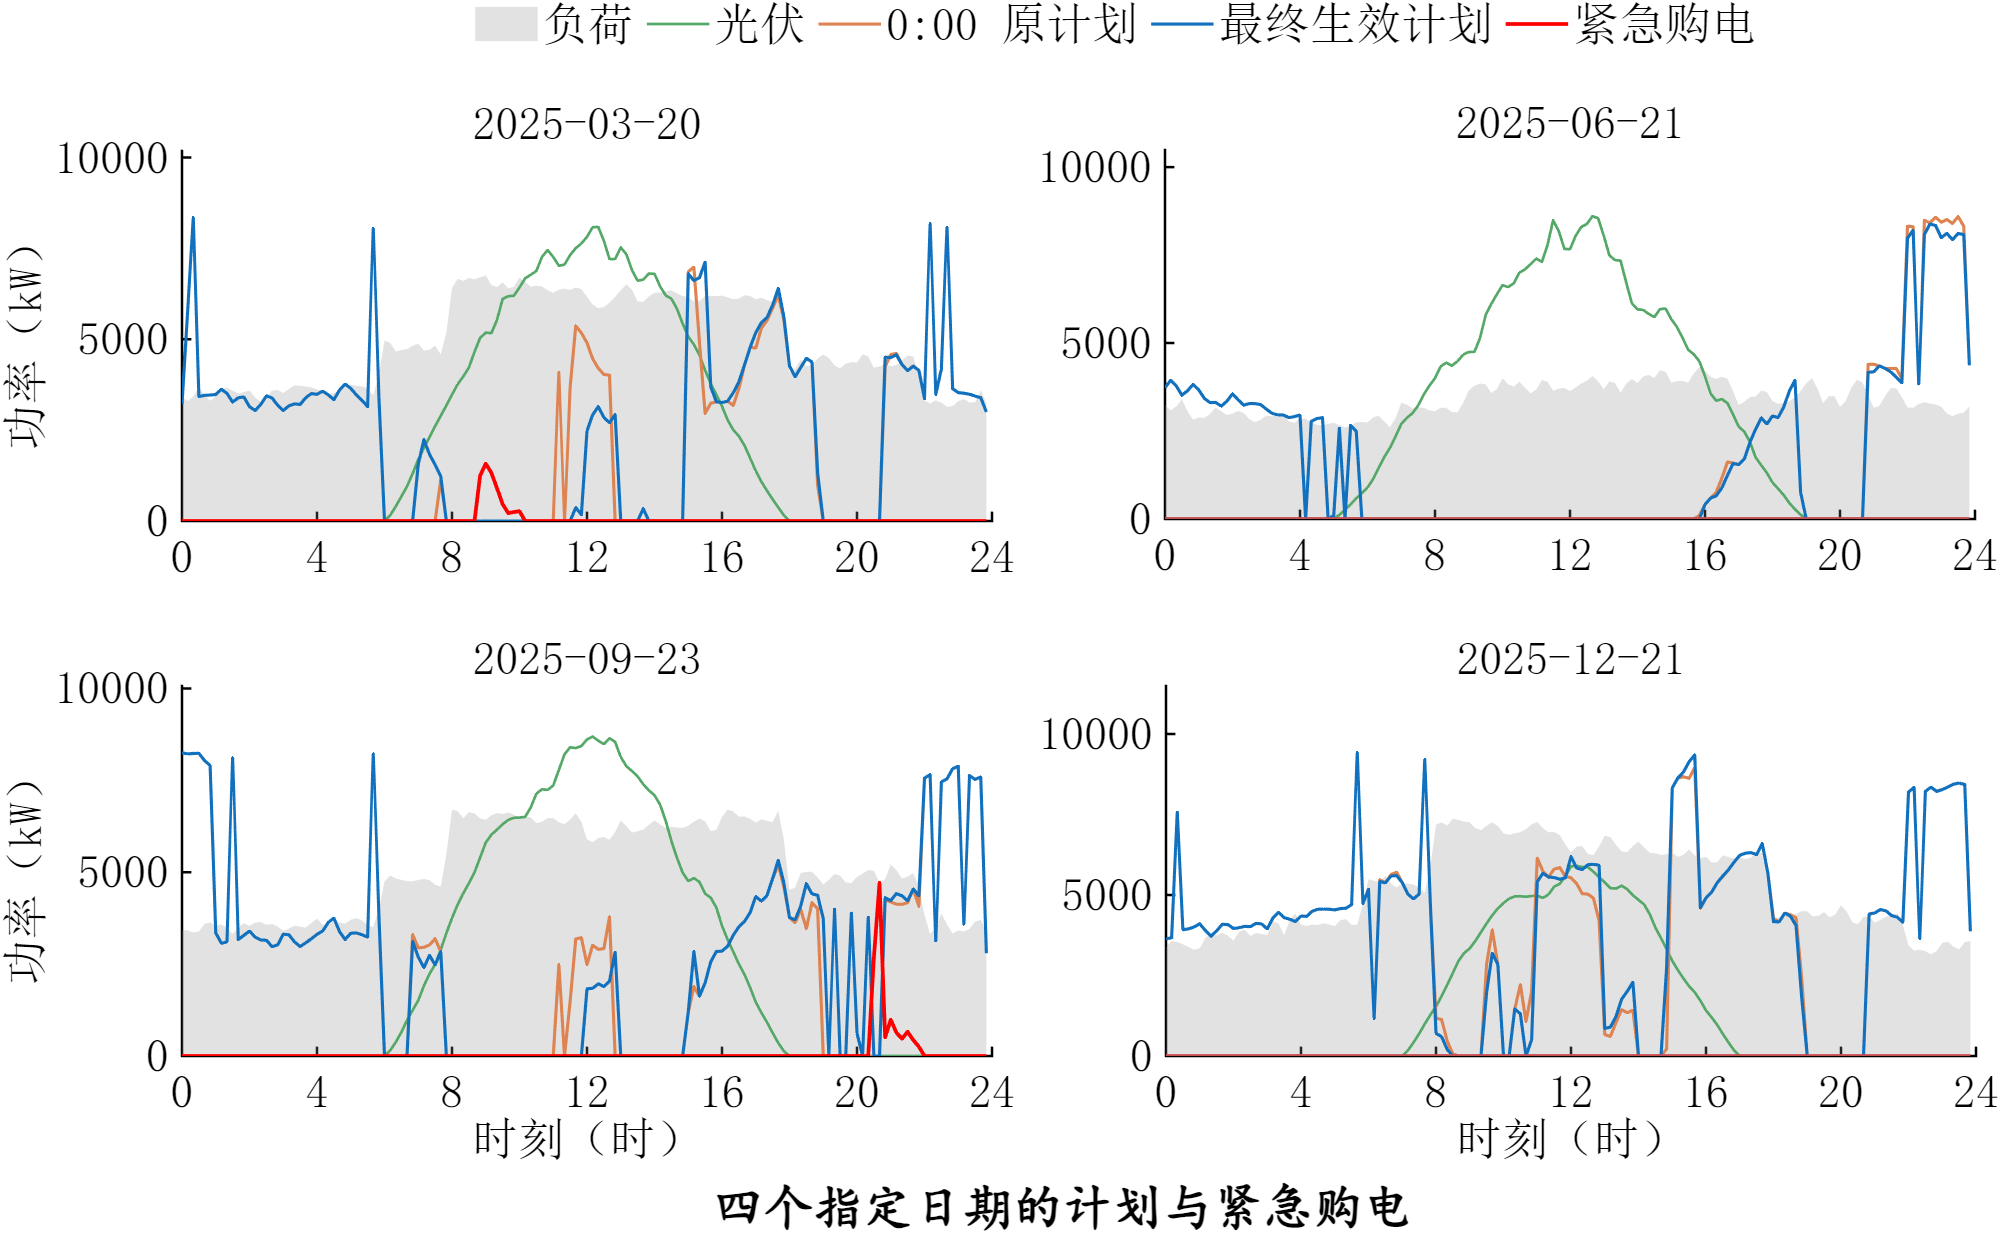
\includegraphics[width=0.78\textwidth,height=0.26\textheight,keepaspectratio]{figures/q3_stages.png}
\caption{问题三四个指定日期的四阶段计划轨迹与紧急购电（电量单位：kWh）}
\label{fig:q3-stage}
\end{figure}

再调整的方向与幅度逐日不同：03-20 与 06-21 为净调减，09-23 与 12-21 为净调增，说明模型确实在利用日内预报修正偏差，而不是单向动作。
%FIG:END q3-stage

%FIG:BEGIN q3-soc
问题三日末储电量的全年轨迹见图~\ref{fig:q3-soc}。

\begin{figure}[htbp]
\centering
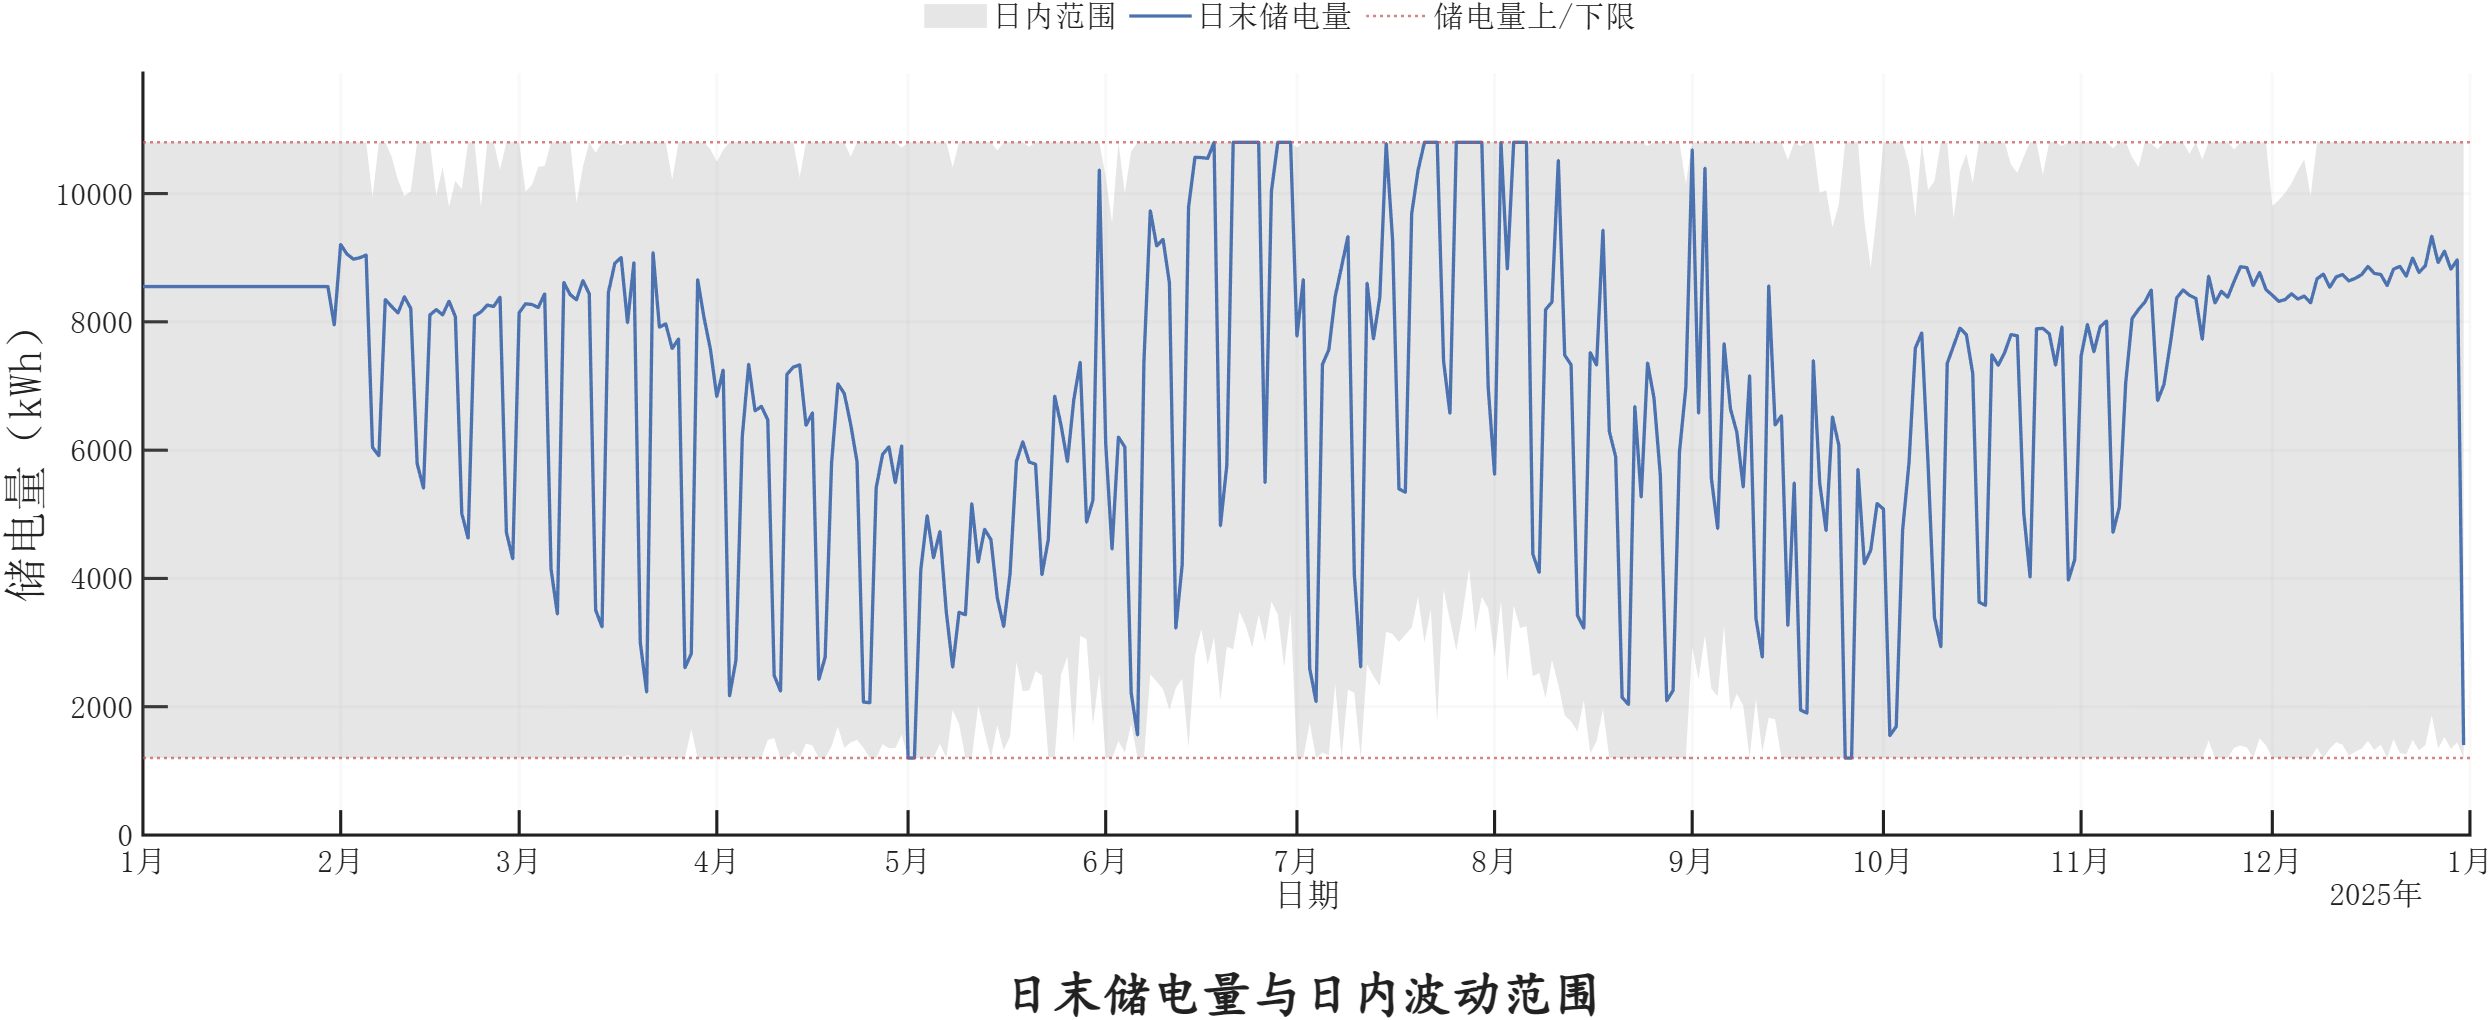
\includegraphics[width=0.78\textwidth,height=0.26\textheight,keepaspectratio]{figures/q3_soc.png}
\caption{问题三报送窗口内日末储电量轨迹（电量单位：kWh）}
\label{fig:q3-soc}
\end{figure}

报送窗口内日末储电量均值为 6\,848 kWh，仅 4 天触及下限（问题二为 1 天）。触底天数增加是日内多次重优化的代价，但储能运行整体仍保持平稳。
%FIG:END q3-soc

\subsection{模型检验}

程序应至少检查：

校验覆盖时间索引一致性、附件 3 预测映射与线性插值、无未来信息泄漏与非预见性、阶段边界不回改、阶段初值取真实储电量、能量平衡与储能递推、充放电互斥、计划电守恒，并以手算样例核对调整费用、确认多次临时调整只结算最终版本；\(S_0\sim S_3\) 各自独立完成全年模拟，且阶段执行与最终拼接结果重放一致。

最大等式残差：

\[
2.39\times10^{-9}.
\]

最大拼接重放偏差：

\[
0.
\]

稳定性分析比较 \(K=4\) 与 \(K=8\)：

\begin{table}[H]
\centering
\zihao{5}
\begin{tabular}{lrrr}
\toprule
指标 & \(K=4\) & \(K=8\) & 相对差异 \\
\midrule
总费用 & 14485230.30 & 14375420.41 & $-0.76\%$ \\
紧急购电量 & 185523.91 & 176950.08 & $-4.62\%$ \\
调整总量 & 8884281.45 & 7223350.14 & $-18.70\%$ \\
\bottomrule
\end{tabular}
\caption{问题三情景数稳定性对照（K=4 与 K=8）}
\label{tab:10}
\end{table}
